A recent survey by Nahim, Khan, and Ju, \hyperlink{ref:1}{A Survey of Flow Matching in Reinforcement Learning} (TMLR, 2026), organizes the field along two axes: \emph{what} the flow models (actions, critics, dynamics) and \emph{where} the RL signal enters (energy-weighted regression, policy gradients through the ODE, GRPO-style objectives). It is a useful map. This note examines one family that the survey does not treat as a group.

At the center are methods that leave the velocity field untouched. They keep a pretrained flow or diffusion policy frozen and train a small network that decides \textbf{which noise to feed it}. Given a state $s$, a proposer picks a point $w$ in noise space, and the frozen generator turns $w$ into an action. Consider a robot policy that sometimes reaches around an obstacle on the left and sometimes on the right. Steering the noise changes how often it chooses each route, while reusing the generator that produces the movements.

The survey already covers an important relative. Its offline section discusses ReFORM (\hyperlink{ref:13}{Zhang et al., 2026}), which manipulates noise inside a bounded support so that the composed policy stays within the learned behavior model's support. Its discussion of ``freezing the flow and learning a correction'' covers policies that \emph{edit the action after it is generated}. DSRL (\hyperlink{ref:2}{Wagenmaker et al., 2025}) and related methods that \emph{choose the input} instead of editing the output are absent. This note follows that thread, including a few neighbors that also train the decoder or learn from corrections rather than rewards.

The note makes two points and then checks them on a small example.

\begin{enumerate}
\item A \textbf{VAE-style inference view} connects the methods. The noise proposer plays the role of an encoder and the frozen generator that of a decoder. For a KL-regularized objective, this becomes an exact variational identity, with value taking the place of reconstruction quality. Other methods share the architecture without optimizing that same objective.
\item The most useful question to ask of each method is \textbf{where RL takes effect}. Action-space data can train a critic directly, but the proposer lives in noise space. Each method is defined largely by how it carries value from one space to the other.
\item A \textbf{two-dimensional experiment} (Section~\ref{sec:4}) trains the same noise proposer with five different ways of carrying value, so one can watch the noise move and the actions follow.
\end{enumerate}

\begin{figure}[htbp]
\centering
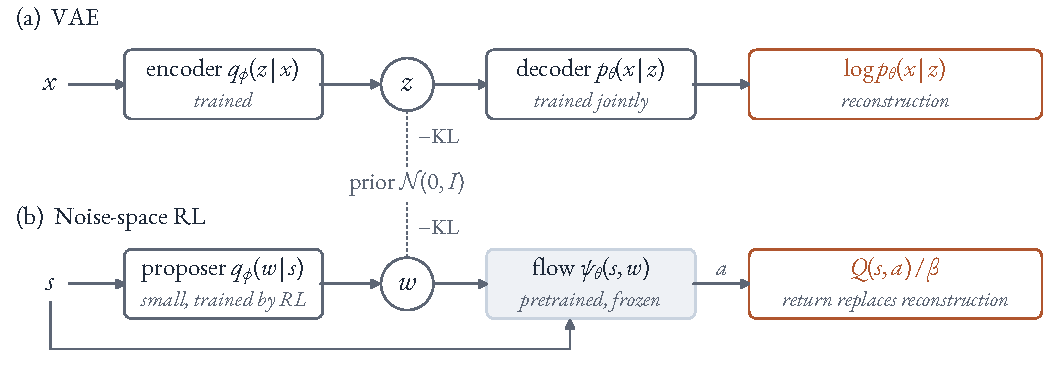
\includegraphics[width=\linewidth]{figures/vae-correspondence.pdf}
\caption{The shared encoder--decoder pattern. (a) A VAE trains an encoder and a decoder jointly to reconstruct its input. (b) In noise-space RL, a proposer $q_\phi$ chooses the noise $w$ for a state $s$, and a pretrained, frozen flow $\psi_\theta$ decodes it into an action. Both latents are pulled toward the same prior $\mathcal{N}(0, I)$ by a KL term. The decoder in (b) produces an action rather than a reconstruction, and value $Q/\beta$ takes the place of the reconstruction term. The correspondence is between objectives (Section~\ref{sec:2}), not between generative models.}
\label{fig:vae-correspondence}
\end{figure}

\section{Setup and notation}
\label{sec:1}
A flow-matching policy learns a velocity field $v_\theta(x, t, s)$ that transports Gaussian noise at time $t = 0$ to actions at $t = 1$. To act, one draws $w \sim \mathcal{N}(0, I)$ and integrates $\dot x_t = v_\theta(x_t, t, s)$ from $x_0 = w$, usually with a few Euler steps,

\begin{equation}
x_{k+1} = x_k + \Delta t\, v_\theta(x_k, t_k, s), \qquad t_k = k\,\Delta t, \quad \Delta t = 1/K, \quad k = 0, \dots, K-1,
\end{equation}
and outputs $a = x_K$. Run with any deterministic sampler (this Euler scheme, the probability-flow ODE of a diffusion policy, DDIM with zero variance, or a one-step distilled model), the policy becomes a fixed map

\begin{equation}
a = \psi_\theta(s, w), \qquad w \sim \mathcal{N}(0, I),
\end{equation}
and all of its randomness enters through $w$. Table~\ref{tab:notation} collects the notation used in the rest of the note; the decoder parameters $\theta$ are pretrained and stay frozen, and only the proposer parameters $\phi$ are learned.

\begin{table}[htbp]
\centering\small
\caption{Notation. The decoder parameters $\theta$ are pretrained and frozen; only the proposer parameters $\phi$ are learned.}
\label{tab:notation}
\begin{tabularx}{\linewidth}{@{}p{0.2\linewidth}>{\raggedright\arraybackslash}X@{}}
\toprule
Symbol & Meaning \\
\midrule
$s,\ a$ & state and action (for robot policies, often a chunk of future actions) \\
$w \in \mathbb{R}^{d}$ & noise fed to the generator; for flow policies, $d$ equals the action dimension \\
$v_\theta,\ K$ & velocity field of the pretrained flow, and the number of sampler steps \\
$\psi_\theta(s, w)$ & the \textbf{decoder}: the deterministic sampler that maps noise $w$ to action $a$ \\
$f_{\#}\mu$ & pushforward: the distribution of $f(x)$ when $x \sim \mu$ \\
$\pi_{\text{base}}(\cdot \mid s)$ & the pretrained policy, $\psi_\theta(s, \cdot)_{\#}\, \mathcal{N}(0, I)$ \\
$q_\phi(w \mid s)$ & the \textbf{noise proposer} (encoder), usually a state-conditioned Gaussian \\
$\pi_\phi(\cdot \mid s)$ & the steered policy, $\psi_\theta(s, \cdot)_{\#}\, q_\phi(\cdot \mid s)$ \\
$Q(s, a)$ & an action-value estimate (critic) \\
$\beta > 0$ & temperature: weight of the KL penalty that keeps $q_\phi$ near $\mathcal{N}(0, I)$ \\
$q^\star,\ \pi^\star$ & the optimal tilted noise distribution and policy, defined in Section~\ref{sec:2} \\
\bottomrule
\end{tabularx}
\end{table}

A noise-space method keeps $\theta$ fixed and replaces only the distribution of the input, from $\mathcal{N}(0, I)$ to $q_\phi(\cdot \mid s)$. The proposer can be a Gaussian with a state-dependent mean and variance, a deterministic map, a residual added to fresh noise, or even a single constant vector. It is usually smaller than the generator, though not necessarily tiny: Noise PPO uses a roughly 187M-parameter proposer. The decoder can be very large (DSRL steers $\pi_0$, a 3.3B-parameter generalist policy) and is never updated.

DSRL states the construction cleanly. Define a new MDP whose actions are noises:

\begin{equation}
P^{W}(\cdot \mid s, w) = P(\cdot \mid s, \psi_\theta(s, w)), \qquad r^{W}(s, w) = r(s, \psi_\theta(s, w)).
\end{equation}
The diffusion policy becomes part of the environment. Any RL algorithm can now run over $w$, using only forward passes of the generator, without its weights or its intermediate denoising steps.

The idea is older than diffusion policies. PLAS (\hyperlink{ref:4}{Zhou et al., 2020}) learned a policy in the latent space of a conditional VAE for offline RL. PARROT (\hyperlink{ref:3}{Singh et al., 2021}) trained a normalizing-flow behavioral prior and ran RL on its noise. It compared directly against a conditional-VAE latent space and argued that invertibility lets the agent keep full control over the final action. DSRL singles out PARROT as the precedent in control and makes the same point from the other side: diffusion models are not invertible by construction, so it is ``much less clear'' that steering their noise is expressive enough. Empirically, DSRL finds that it is.

\section{Reading it as a VAE}
\label{sec:2}
Recall the evidence lower bound of an ordinary VAE (\hyperlink{ref:21}{Kingma \& Welling, 2014}); a conditional VAE additionally conditions its distributions on context:

\begin{equation}
\log p(x) \;\ge\; \mathbb{E}_{q_\phi(z \mid x)}\big[\log p_\theta(x \mid z)\big] \;-\; \mathrm{KL}\big(q_\phi(z \mid x) \,\Vert\, p(z)\big).
\end{equation}
To make the connection precise, consider the following KL-regularized policy-improvement objective:

\begin{equation}
J(\phi) = \mathbb{E}_{s}\Big[\, \mathbb{E}_{w \sim q_\phi(\cdot \mid s)}\, Q\big(s, \psi_\theta(s, w)\big) \;-\; \beta\, \mathrm{KL}\big(q_\phi(\cdot \mid s) \,\Vert\, \mathcal{N}(0, I)\big) \Big].
\end{equation}
Here $Q$ is held fixed during the proposer update, and states are sampled from a fixed training distribution. This is a local improvement objective, not by itself a complete solution to sequential RL. Table~\ref{tab:vae} lines up the two expressions term by term.

\begin{table}[htbp]
\centering\small
\caption{Correspondence between the terms of a VAE and KL-regularized noise-space RL.}
\label{tab:vae}
\begin{tabularx}{\linewidth}{@{}>{\raggedright\arraybackslash}X>{\raggedright\arraybackslash}X@{}}
\toprule
VAE & Noise-space RL \\
\midrule
observed input $x$ & desired optimality, with state $s$ as context \\
encoder $q_\phi(z \mid x)$ & noise proposer $q_\phi(w \mid s)$ \\
prior $p(z) = \mathcal{N}(0, I)$ & the Gaussian the flow was trained from \\
decoder $p_\theta(x \mid z)$ & frozen flow $\psi_\theta(s, w)$ \\
reconstruction $\log p_\theta(x \mid z)$ & value $Q(s, \psi_\theta(s, w)) / \beta$ \\
KL to the prior & KL to $\mathcal{N}(0, I)$: penalize departure from the training prior \\
decoder trained jointly & decoder pretrained by imitation, usually frozen \\
\bottomrule
\end{tabularx}
\end{table}

The exact connection is a variational identity. Define $Z(s) = \mathbb{E}_{w \sim \mathcal{N}(0,I)}[\exp(Q(s, \psi_\theta(s,w))/\beta)]$ and assume it is finite. Then, for each state,

\begin{equation}
\log Z(s) = \underbrace{\mathbb{E}_{q_\phi}[Q(s, \psi_\theta(s,w))/\beta] - \mathrm{KL}(q_\phi \Vert \mathcal{N}(0,I))}_{J(\phi;\, s)/\beta} + \mathrm{KL}(q_\phi \Vert q^\star).
\end{equation}
The last term is nonnegative, so the first two terms form a lower bound. In the control-as-inference view (\hyperlink{ref:22}{Levine, 2018}), this can be read as an ELBO for a desired ``optimality'' observation. When $Q$ is bounded above, a state-dependent scaling makes the exponential a valid binary likelihood; the variational identity itself needs only a finite $Z(s)$. The unrestricted best proposer is

\begin{equation}
q^\star(w \mid s) = \frac{\mathcal{N}(w; 0, I)\, \exp\big(Q(s, \psi_\theta(s, w))/\beta\big)}{Z(s)}.
\end{equation}
Writing $J(\phi; s)$ for the term inside the outer expectation of $J$, the identity also gives a ruler: for any proposer, $\log Z(s) - J(\phi; s)/\beta = \mathrm{KL}(q_\phi \Vert q^\star)$ measures how far it is from the best one. Section~\ref{sec:4} uses it.

The difference from an ordinary VAE is what counts as the observation. The encoder is not asked to explain an action that was seen. It is asked to infer which noise \emph{would have produced a good action}. The evidence is desired success, represented here by the value estimate. This is why ``VAE-style'' is more accurate than calling every method a conditional VAE. A deterministic proposer, for example, has infinite KL to a continuous Gaussian; box constraints, spherical latents, and supervised inversion require their own objectives.

Two facts make this reading useful. \hyperlink{ref:6}{Eyring et al. (2025)} state both for distilled text-to-image generators, and both carry over to policies without change.

\begin{proposition}[Tilting the noise tilts the policy]\label{prop:tilt}
Pushing the noise posterior through the frozen decoder gives exactly the reward-tilted base policy:

\begin{equation}
\psi_\theta(s, \cdot)_{\#}\, q^\star(\cdot \mid s) \;=\; \pi^\star(\cdot \mid s) \;\propto\; \pi_{\text{base}}(\cdot \mid s)\, \exp\big(Q(s, \cdot)/\beta\big).
\end{equation}
\end{proposition}
The reason is that the tilt depends on $w$ only through $a = \psi_\theta(s, w)$.

\begin{proof}[Proof of Proposition~\ref{prop:tilt}]
For a bounded test function $f$, suppressing the fixed state $s$,
\begin{equation*}
\begin{aligned}
\mathbb{E}_{q^\star}[f(\psi_\theta(w))]
&= Z^{-1}\mathbb{E}_{w\sim\mathcal{N}(0,I)}
   [f(\psi_\theta(w))e^{Q(\psi_\theta(w))/\beta}] \\
&= Z^{-1}\mathbb{E}_{a\sim\pi_{\text{base}}}
   [f(a)e^{Q(a)/\beta}].
\end{aligned}
\end{equation*}
\end{proof}

No invertibility is needed. This is the same target that KL-regularized fine-tuning of the whole flow aims for, but a small proposer can only approximate it as well as its distribution family and optimization allow. A single Gaussian, for example, need not represent a multimodal noise posterior. Figure~\ref{fig:tilt-noise-tilts-policy} shows the target on a 2D example.

\begin{figure}[htbp]
\centering
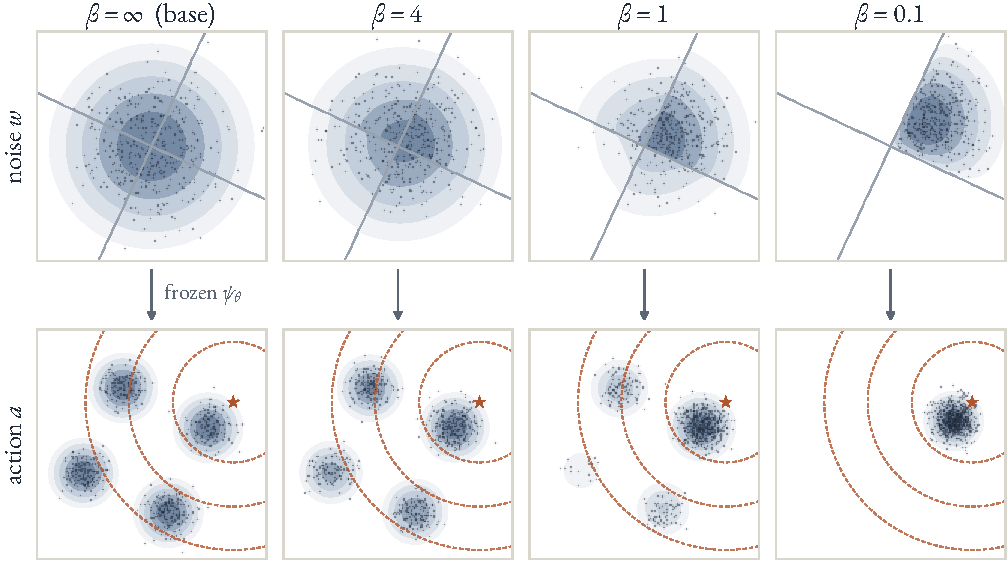
\includegraphics[width=\linewidth]{figures/tilt-noise-tilts-policy.pdf}
\caption{Tilting the noise tilts the policy (exact, no learning). The base policy is a four-cluster mixture in a 2D action space, and $\psi$ is the exact flow-matching ODE map onto it. Each column is one value of $\beta$. Top: the tilted noise distribution $q^\star(w) \propto \mathcal{N}(w; 0, I)\, e^{Q(\psi(w))/\beta}$ (shading) and samples from it (dots); grey lines split the noise plane into the four regions that decode to the four clusters. Bottom: the same samples after the frozen flow, over the tilted policy $\pi_{\text{base}}\, e^{Q/\beta}$ (shading); dashed circles are contours of $Q$, and the star marks its peak. At $\beta = \infty$ the base policy is recovered. As $\beta$ shrinks, probability moves to the cluster nearest the peak, but no new cluster appears.}
\label{fig:tilt-noise-tilts-policy}
\end{figure}

\begin{proposition}[The noise-space KL is a conservative proxy]\label{prop:dpi}
By the data processing inequality,

\begin{equation}
\mathrm{KL}\big(\pi_\phi(\cdot \mid s) \,\Vert\, \pi_{\text{base}}(\cdot \mid s)\big) \;\le\; \mathrm{KL}\big(q_\phi(\cdot \mid s) \,\Vert\, \mathcal{N}(0, I)\big),
\end{equation}
\end{proposition}
with equality when $\psi_\theta(s, \cdot)$ is invertible. The left side can be expensive to evaluate: a continuous normalizing flow can compute densities through divergence integration, while a generic distilled decoder need not offer a tractable density. For a Gaussian proposer $\mathcal{N}(\mu, \mathrm{diag}\,\sigma^2)$, the right side is the familiar VAE term $\tfrac12 \sum_j (\mu_j^2 + \sigma_j^2 - 1 - \log \sigma_j^2)$. Noise PPO (\hyperlink{ref:5}{Miao et al., 2025}) uses exactly this KL penalty, together with an entropy bonus. Noise Hypernetworks and LP-DS (\hyperlink{ref:11}{Simsir \& Oguz, 2026}) write the steered noise as a residual $w = \epsilon + \Delta$ and approximate the KL by $\tfrac12\, \mathbb{E}\Vert\Delta\Vert^2$, a surrogate justified under regularity and small-Jacobian assumptions. Bounding the residual's magnitude alone does not establish those assumptions.

\section{Where RL takes effect: carrying value into noise space}
\label{sec:3}
The decision variable for RL is now the noise. Much of the available supervision, however, lives in the other space. An action-space critic $Q(s, a)$ is ordinary temporal-difference learning on $(s, a, r, s')$ transitions, and offline datasets, demonstrations, and human corrections all come labeled with actions, not noises. The proposer needs a value of $w$, or a gradient with respect to $w$, of the composition

\begin{equation}
w \;\longmapsto\; Q\big(s, \psi_\theta(s, w)\big).
\end{equation}
This simplifies the policy interface but not necessarily the optimization: nearby noises may have very different values. So the central design question of the family is how to \textbf{carry an action-space value back into noise space}. The papers suggest five routes, summarized in Figure~\ref{fig:five-routes}. They are not disjoint categories: Route 4 is a special case of Route 3, and a method can combine inversion with a noise critic. What separates them is what each needs from the decoder: forward calls only, an inverse, or derivatives.

\begin{figure}[htbp]
\centering
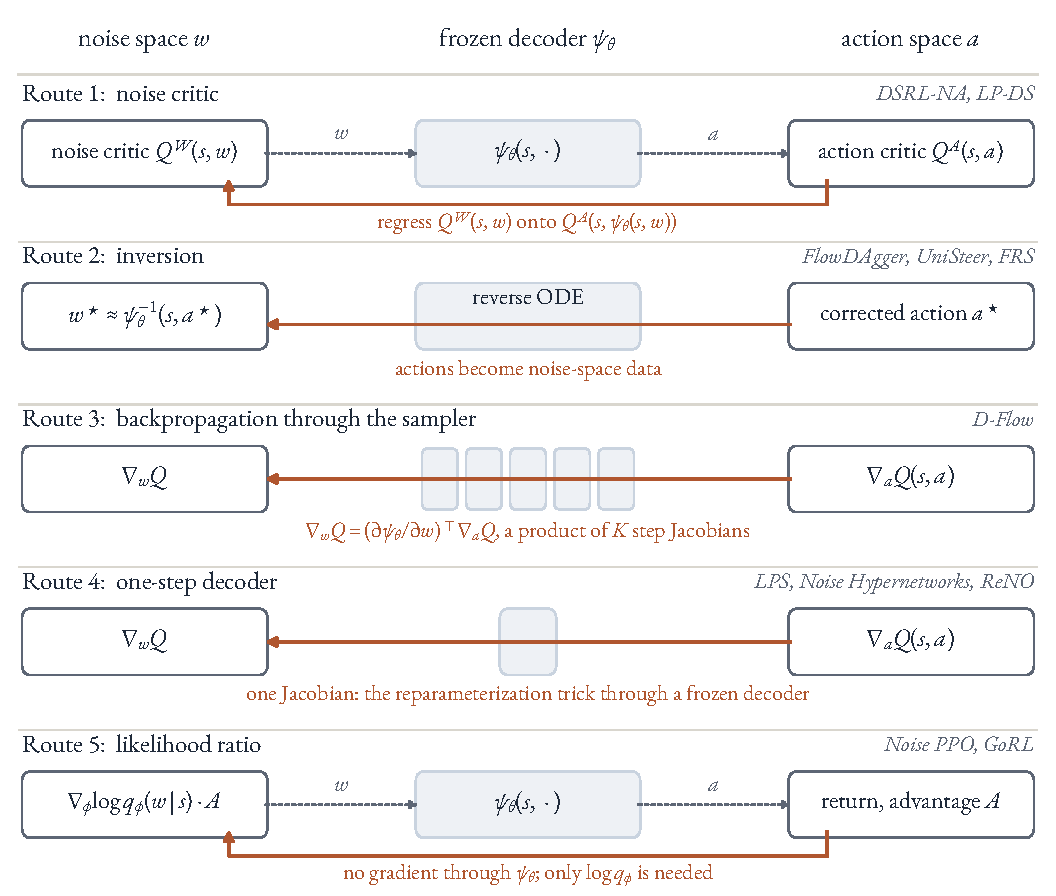
\includegraphics[width=0.82\linewidth]{figures/five-routes.pdf}
\caption{Five routes for training the noise proposer. In each row, noise space is on the left, the frozen decoder in the middle, and action space on the right. Grey dashed arrows are forward decoding; orange arrows show what crosses back into noise space. Route 1 is drawn in its two-critic form; Route 2 uses action supervision rather than a critic; Route 5 uses returns directly. Representative methods are listed at the right of each row.}
\label{fig:five-routes}
\end{figure}

\paragraph{Route 1: learn a critic in noise space.} One option is to learn a noise-space critic directly from rollouts, as in DSRL-SAC. DSRL-NA (``noise-aliased'') instead keeps two critics. It learns $Q^{A}(s, a)$ by temporal-difference learning in action space, then distills it into a noise-space critic by regressing $Q^{W}(s, w)$ onto $Q^{A}(s, \psi_\theta(s, w))$ with $w \sim \mathcal{N}(0, I)$. The decoder is only ever run forward. Because many noises decode to similar actions, a noise that was never played can still receive an accurate value. On Robomimic Square, plain SAC in noise space (DSRL-SAC) needs about twice as many samples. On real robots, DSRL reports cases where success rose from 20\% to 90\% within fewer than 50 online episodes. LP-DS keeps the same two-critic design. A related forward-only idea appears in GoldenStart (\hyperlink{ref:10}{Zhang et al., 2026}), which picks the highest-value noise for each state by decoding candidates and scoring them with the critic, then fits a conditional VAE to these noises as a learned prior. GoldenStart is not a pure frozen-decoder method, though: its flow teacher keeps training, and the deployed policy is a distilled one-step student. \emph{Cost:} a second approximation. LPS argues that a distilled critic can match values well and still point its gradient in the wrong direction.

\paragraph{Route 2: invert the flow and move the data.} Sometimes the signal is an action rather than a reward: a human correction, or a coarse suggestion from a vision-language model. A flow can be integrated backwards to recover the noise that would have produced that action, $w^\star \approx \psi_\theta^{-1}(s, a^\star)$, and the corrected actions become noise-space training targets. A generic VAE decoder has no inverse, so it relies on a learned encoder for inference. An exact ODE flow is invertible under suitable regularity assumptions; a coarse numerical sampler or a distilled decoder need not be. FlowDAgger (\hyperlink{ref:14}{Murray et al., 2026}) regresses the proposer onto inverted corrections. UniSteer (\hyperlink{ref:15}{Lu et al., 2026}) stores inverted transitions $(s, \hat w, r, s')$ in both a demonstration buffer and an RL buffer, and trains a noise-space critic on them by ordinary TD learning. Flow Reversal Steering (\hyperlink{ref:16}{Tang et al., 2026}) maps coarse reference actions to nearby modes of a generalist policy, then distills them or uses them to bootstrap DSRL. Inversion supplies a noise that reconstructs the correction, not a sample from the reward-tilted posterior above. \emph{Cost:} inversion error. With the short ODE schedules of robot action heads, a naive reverse Euler step is not accurate enough, which is why FlowDAgger and UniSteer both use per-step fixed-point refinement for their flow action heads. Convergence requires conditions such as a step size small relative to the velocity field's Lipschitz constant; it is not automatic.

\paragraph{Route 3: backpropagate through the sampling iterations.} The chain rule gives the noise gradient exactly:

\begin{equation}
\nabla_w\, Q\big(s, \psi_\theta(s, w)\big) = \Big(\frac{\partial \psi_\theta}{\partial w}\Big)^{\!\top} \nabla_a Q(s, a),
\end{equation}
\begin{equation}
\frac{\partial \psi_\theta}{\partial w} = \prod_{k=K-1}^{0} \Big(I + \Delta t\, \frac{\partial v_\theta}{\partial x}(x_k, t_k, s)\Big)
\end{equation}
for the $K$-step Euler sampler of Section~\ref{sec:1}, with later-step Jacobians multiplying on the left. ``Exact'' here means the derivative of the implemented sampler and learned critic, not of the true environment return. With a reparameterized proposer $w = \mu_\phi(s) + \sigma_\phi(s) \odot \epsilon$, this is the VAE reparameterization trick with a frozen decoder, and no second critic is needed. D-Flow (\hyperlink{ref:8}{Ben-Hamu et al., 2024}) takes this route for per-sample noise optimization in image, audio, and molecule generation. \emph{Cost:} the gradient has to pass through every step of the solver. DSRL calls this ``computationally intensive and numerically unstable'', and LPS calls it ``expensive and unstable''.

\paragraph{Route 4: make the decoder one step.} If $\psi_\theta$ is a single network evaluation, the product above has a single factor, and the critic gradient reaches the noise in one backward pass. LPS (\hyperlink{ref:12}{Im et al., 2026}) uses a one-step MeanFlow base policy for exactly this reason, and backpropagates $\nabla_a Q$ straight into the latent actor without a noise-space critic. It is a useful architectural neighbor rather than a strictly frozen-decoder method: its Algorithm 1 also updates the base policy by imitation during training. ReNO does the same with reward models on one-step image generators, and Noise Hypernetworks on distilled one- or few-step generators (SD-Turbo, SANA-Sprint, FLUX-Schnell). With a few steps the chain in Route 3 is short rather than trivial, which is still cheap. \emph{Cost:} the base policy must be one-step, which usually means it was trained or distilled for that purpose.

\paragraph{Route 5: skip the transfer.} The likelihood-ratio gradient of the return term, $\mathbb{E}\big[\nabla_\phi \log q_\phi(w \mid s)\, A(s, w)\big]$ with an advantage estimate $A$, needs only $\log q_\phi$, which is exact for a Gaussian proposer: no ODE divergence, no SDE conversion, no surrogate likelihood. Much of the survey's online-RL section is about recovering a usable likelihood for flow policies; in noise space the problem does not arise. Noise PPO treats text-to-image generation as a one-step MDP whose action is the initial noise, and runs PPO with sampled rewards; KL and entropy regularizers contribute additional gradient terms. \emph{Cost:} the usual variance of score-function estimates.

\section{A two-dimensional experiment}
\label{sec:4}
To see the five routes at work, we train the same noise proposer with each of them on a toy problem small enough to plot and to evaluate exactly. Code for this section and all figures is available \href{https://github.com/yuhanchi/yuhanchi.github.io/tree/main/\_src/choose-the-noise}{on GitHub}.

\paragraph{Setup.} Actions are points $a \in \mathbb{R}^2$. The base policy imitates the four-cluster mixture of Figure~\ref{fig:tilt-noise-tilts-policy}: a small velocity network (an MLP) is trained once by conditional flow matching and then frozen, and the decoder $\psi_\theta$ is its $K = 10$-step Euler sampler. The pushforward of $\mathcal{N}(0, I)$ through it puts between 24.9\% and 25.1\% of its mass on each cluster. A state is a goal angle $s \in [0, 2\pi)$, and the critic is known exactly: $Q(s, a) = -\tfrac12 \Vert a - g(s) \Vert^2$, where the goal $g(s)$ lies on the circle through the cluster centers. With $\beta = 1$, a goal between two clusters makes $q^\star$ bimodal. The proposer is a Gaussian $\mathcal{N}(\mu_\phi(s), \mathrm{diag}\,\sigma_\phi(s)^2)$ whose mean and log standard deviation come from a small MLP, initialized at the prior $\mathcal{N}(0, I)$.

Because $Q$ is given, the experiment isolates the transfer step: there is no TD learning and no exploration. The ruler from Section~\ref{sec:2} measures the result: $\mathrm{KL}(q_\phi \Vert q^\star) = \log Z(s) - J(\phi; s)/\beta$, estimated by Monte Carlo and averaged over 64 evenly spaced states.

\paragraph{How the noise moves.} Figure~\ref{fig:experiment-training} follows one state during training with Route 3. The proposer starts as the prior, so the actions are the base policy. Within a few dozen updates, the noise cloud shrinks and slides into the region of noise space that decodes to the cluster nearest the goal; the actions follow it without any change to the decoder.

In this state the goal lies between two clusters, so the target policy is bimodal. One Gaussian is nonetheless enough to reach both: the two clusters decode from adjacent regions of noise space, and the proposer settles across their shared boundary. \textbf{A distribution that is bimodal in action space can be unimodal in noise space.} What the Gaussian cannot match is the shape of $q^\star$, which is cut off sharply along the grey lines; a few of its samples also still decode to the two far clusters. The remaining $\mathrm{KL}(q_\phi \Vert q^\star)$ at this state is about 0.17 nats.

\begin{figure}[htbp]
\centering
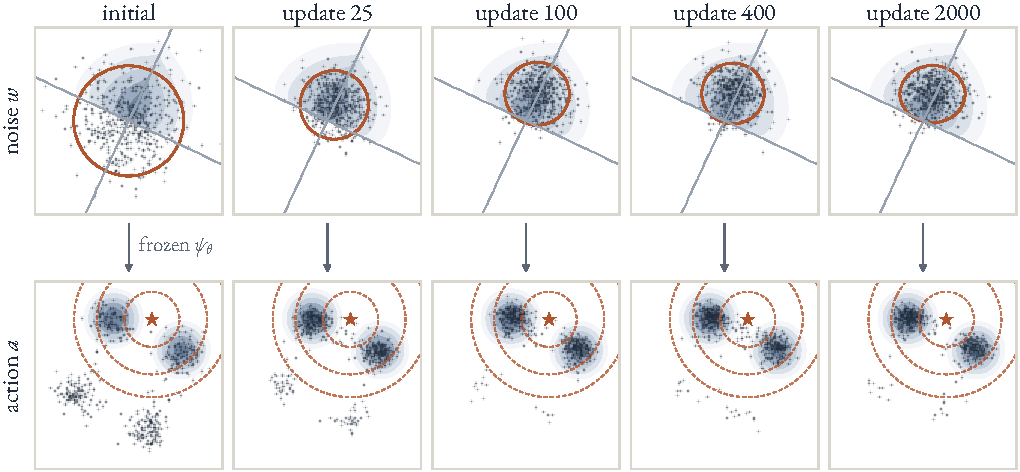
\includegraphics[width=\linewidth]{figures/experiment-training.pdf}
\caption{Learning which noise to choose, for one state (goal angle 67.5$^\circ$) with Route 3. Columns are snapshots during training. Top: samples from the proposer $q_\phi(w \mid s)$ (dots) and its two-standard-deviation ellipse (orange), over the exact tilted posterior $q^\star$ for the learned decoder (shading); grey lines separate the noise regions that decode to different clusters. Bottom: the same samples after the frozen 10-step decoder, over the tilted target policy $\pi_{\text{base}}\, e^{Q/\beta}$ (shading, computed from the mixture the flow imitates); the star is the goal and dashed circles are contours of $Q$. The decoder never changes; only the noise does.}
\label{fig:experiment-training}
\end{figure}

\paragraph{Comparing the routes.} Each route trains the same proposer for 2,000 updates, each on 1,024 decoded noises (256 states with 4 noises each), and is run with three seeds. Routes 1, 3, 4, and 5 maximize the objective $J$ of Section~\ref{sec:2}, using a distilled noise critic, gradients through the 10 Euler steps, gradients through a one-step decoder distilled from the 10-step sampler, and a likelihood-ratio gradient with a leave-one-out baseline. Route 2 never sees $Q$. It receives ``corrected'' actions sampled from the tilted target policy, a stand-in for an expert, inverts them through the decoder by fixed-point iteration, and fits the proposer to the recovered noises by maximum likelihood. Table~\ref{tab:routes} and Figure~\ref{fig:experiment-routes} summarize the outcome.

\begin{table}[htbp]
\centering\small
\caption{Five routes on the 2D toy. $\mathrm{KL}(q_\phi \Vert q^\star)$ is averaged over 64 states (mean $\pm$ standard deviation over three seeds; lower is better). Time is the median wall-clock time per update on a laptop GPU (RTX 5060), including Python overhead. Route 4 is measured against the posterior of its own one-step decoder.}
\label{tab:routes}
\begin{tabularx}{\linewidth}{@{}>{\raggedright\arraybackslash}p{0.27\linewidth}>{\raggedright\arraybackslash}Xcc@{}}
\toprule
Route & Needs from the decoder & $\mathrm{KL}(q_\phi \Vert q^\star)$ & ms / update \\
\midrule
1. noise critic & forward calls & 0.207 $\pm$ 0.004 & 8.6 \\
2. inversion & an inverse (20 fixed-point iterations per step) & 0.312 $\pm$ 0.007 & 60.2 \\
3. backprop through 10 steps & derivatives & 0.211 $\pm$ 0.002 & 7.2 \\
4. one-step decoder & derivatives of a distilled one-step student & 0.206 $\pm$ 0.002 & 2.9 \\
5. likelihood ratio & forward calls & 0.211 $\pm$ 0.003 & 5.6 \\
reference: best Gaussian for each state separately & derivatives & 0.198 & --- \\
\bottomrule
\end{tabularx}
\end{table}

\begin{figure}[htbp]
\centering
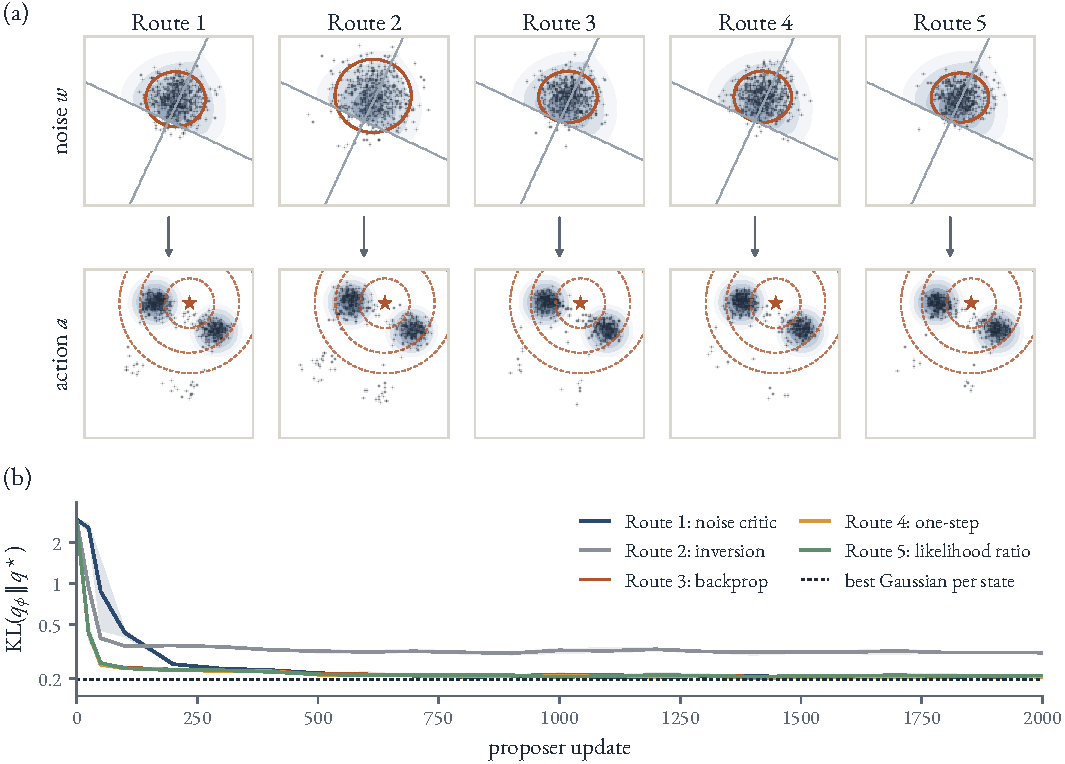
\includegraphics[width=\linewidth]{figures/experiment-routes.pdf}
\caption{Five routes, one proposer. (a) The final proposer of each route for the same state as Figure~\ref{fig:experiment-training}, drawn as in Figure~\ref{fig:experiment-training} (seed 0). (b) $\mathrm{KL}(q_\phi \Vert q^\star)$ averaged over 64 states during training; lines are means and bands span three seeds. The dashed line is the best single Gaussian fitted to each state separately.}
\label{fig:experiment-routes}
\end{figure}

Three observations follow.

\begin{itemize}
\item \textbf{The four routes that maximize $J$ end in the same place.} Routes 1, 3, 4, and 5 reach 0.206--0.211 nats, against 0.198 for the best single Gaussian fitted to each state separately. In this toy the remaining error comes from the Gaussian family, not from the transfer route, and amortizing over states costs little.
\item \textbf{They differ in how they get there.} Route 1 starts slowly, because its noise critic has to be learned before its gradient means anything (Figure~\ref{fig:experiment-routes}b). The cost per update spans a factor of twenty: 2.9\,ms through the one-step decoder, 7.2\,ms through ten Euler steps, and 60\,ms for inversion.
\item \textbf{Route 2 settles higher, and not because inversion fails.} Fixed-point inversion reconstructs the corrected actions to a median error of about $10^{-7}$; a single naive reverse Euler pass per step leaves a median error of 0.05, about an eighth of a cluster's standard deviation (0.38). The difference lies in the objective. Maximum likelihood on samples from the target minimizes $\mathrm{KL}(q^\star \Vert q_\phi)$, which favors a wider Gaussian that covers the posterior (Figure~\ref{fig:experiment-routes}a), while the ruler measures $\mathrm{KL}(q_\phi \Vert q^\star)$. Corrections teach the proposer to imitate the target, not to optimize the objective.
\end{itemize}

These numbers come from a deliberately easy setting: two dimensions, an exact critic, and a smooth decoder. They say nothing about critic error, about the variance of Route 5 in high dimensions, or about the instability that DSRL and LPS report for Route 3 with large decoders. What the toy does show is the shape of the problem: the decoder fixes which actions are reachable, the proposer only decides how much noise to send to each region, and a single Gaussian must choose between regions when the target has several.

\section{A map of the family}
\label{sec:5}
Table~\ref{tab:map} groups the methods by their main learning route. It includes related designs with changing decoders, labeled explicitly. ``Prior control'' distinguishes actual constraints from initialization or supervision alone.

\begin{table}[htbp]
\centering\footnotesize
\caption{Noise-space methods and close relatives, grouped by the route through which value reaches the noise. ``Prior control'' distinguishes actual constraints from initialization or supervision alone.}
\label{tab:map}
\begin{tabularx}{\linewidth}{@{}>{\raggedright}p{0.12\linewidth}>{\raggedright}p{0.14\linewidth}>{\raggedright}p{0.17\linewidth}>{\raggedright}X>{\raggedright\arraybackslash}p{0.2\linewidth}@{}}
\toprule
Route & Method & Setting & Proposer $q_\phi(w \mid s)$ & Prior control \\
\midrule
1. noise critic & \hyperlink{ref:3}{PARROT} (2021; preprint 2020) & robot manipulation & RL policy over the noise of an invertible normalizing flow & prior initialization; no lasting proximity guarantee \\
1. noise critic & \hyperlink{ref:2}{DSRL} (2025) & online and offline control; $\pi_0$ & state-conditioned noise actor; SAC, or an action critic distilled into a noise critic & noise box $[-b, b]^d$ \\
1. noise critic & \hyperlink{ref:11}{LP-DS} (2026) & online control; $\pi_0$ & residual $\epsilon + \Delta_\phi(s, \epsilon)$ with noise-aliased critics & Lagrangian trust region on $\mathbb{E}\Vert\Delta\Vert^2$ \\
1. forward scoring & \hyperlink{ref:10}{GoldenStart} (2026) & distilled one-step flow policies; teacher not frozen & conditional VAE fit to the highest-value noise per state & CVAE fitting; entropy control is on the action student \\
2. inversion & \hyperlink{ref:14}{FlowDAgger}, \hyperlink{ref:15}{UniSteer} (2026) & human-in-the-loop VLA adaptation & noise policy regressed onto inverted corrections; UniSteer adds a noise critic & inverted targets; inversion alone does not ensure typical noise \\
2. inversion & \hyperlink{ref:16}{Flow Reversal Steering} (2026) & generalist policies & auxiliary noise policy trained on inverted coarse actions & coarse references guide reversal; no generic KL bound \\
3 / 4. backpropagation & \hyperlink{ref:13}{ReFORM} (2026) & offline RL; BC model and distilled decoder also trained & reflected flow generating bounded input noise & projected steps keep noise inside the source ball \\
4. one-step & \hyperlink{ref:6}{Noise Hypernetworks} (2025) & distilled text-to-image & residual on fresh noise (LoRA), reward gradient through the generator & $\tfrac12\Vert\Delta\Vert^2$ as a KL surrogate \\
4. one-step & \hyperlink{ref:12}{LPS} (2026) & offline RL; real robots; base also trained by imitation & latent actor on a sphere, $\nabla_a Q$ through a one-step MeanFlow & sphere of radius $\sqrt{d}$ \\
5. likelihood ratio & \hyperlink{ref:5}{Noise PPO} (2025) & text-to-image & prompt-conditioned Gaussian trained by PPO & KL to $\mathcal{N}(0, I)$, entropy bonus \\
5. likelihood ratio & \hyperlink{ref:9}{GoRL} (2025) & online control & Gaussian encoder; decoder refit in alternating phases & KL to $\mathcal{N}(0, I)$ \\
search & \hyperlink{ref:17}{Golden Ticket} (2026) & generative robot policies & one constant noise vector found by search & --- \\
\bottomrule
\end{tabularx}
\end{table}

ReFORM spans Routes 3 and 4: its original objective differentiates through the BC flow, and its practical design introduces one-step BC distillation to shorten this path. Its Algorithm 1 also continues fitting the BC model. D-Flow is a per-sample example of Route 3.

Three neighboring lines of work are relevant. PDP (\hyperlink{ref:18}{Zhang et al., 2026}) argues that Gaussian noise is a poorly conditioned control interface. Instead of steering it, PDP trains a literal VAE over whole demonstrations, with a geometry-alignment term, and modulates the denoiser with the resulting low-dimensional code. Condition-dependent source flow matching (\hyperlink{ref:19}{Kim et al., 2026}) and LAFM (\hyperlink{ref:20}{Machado et al., 2026}) learn the prior itself together with the flow at training time, which in VAE terms is a learned prior. D-Flow (\hyperlink{ref:8}{Ben-Hamu et al., 2024}) and ReNO (\hyperlink{ref:7}{Eyring et al., 2024}) optimize the noise separately for each sample instead of training a proposer.

\section{What the VAE view explains}
\label{sec:6}
\paragraph{The decoder fixes the map, not a safety guarantee.} With a frozen decoder, every steered action lies in the image of $\psi_\theta(s, \cdot)$. For finite $Q$ and positive $\beta$, the ideal tilted policy has the same support as the base policy. But support is not the same as likely or reliable behavior: a Gaussian-driven invertible flow can have full support, including actions far from the demonstrations. ReFORM makes a stronger construction by bounding the source support; relating its learned model's support to the dataset still depends on how well that model fits. A truly unreachable action cannot be recovered by steering, while a very unlikely action might be. GoRL (\hyperlink{ref:9}{Zhang et al., 2025}) changes the map itself by training the decoder again. Its decoder starts as an identity-like map. Training then alternates between two phases: optimizing a Gaussian encoder with a KL penalty toward $\mathcal{N}(0, I)$ while the decoder is frozen, and refitting the decoder by flow matching on recent rollouts while the encoder is frozen.

\paragraph{$\beta$ is a dial between the base policy and high-value actions.} For a fixed, well-behaved $Q$, as $\beta \to \infty$ the ideal proposer approaches the prior and the system returns to the base policy. This resembles posterior collapse in a VAE, though here returning to the base can be intentional. As $\beta \to 0$, mass concentrates near maximizers, when they exist. Multiple equally good actions---or multiple noises for one action---can remain; a single point mass is not inevitable. LP-DS reports that prior-replacing steering can lose modes, and uses a residual trust region whose multiplier plays a role similar to $\beta$, for its surrogate penalty. Golden Ticket (\hyperlink{ref:17}{Patil et al., 2026}) imposes a different restriction: one noise vector shared across states. It is not the general low-temperature limit of a state-conditioned proposer.

\paragraph{Holes in the latent space.} A VAE can decode poorly in regions its training rarely visits. A Gaussian-driven flow can have the same problem: most training draws come from typical regions of the Gaussian. The family uses several ways to discourage atypical queries, with different strengths. DSRL bounds each noise coordinate in $[-b,b]$ and reports that $b$ between 1 and 3 works well online. A box bounds coordinates; it does not by itself enforce the Gaussian's typical radius. LPS trains both its base policy and its latent actor on the sphere of radius $\sqrt{d}$, where high-dimensional Gaussian mass concentrates, to prevent what it calls ``norm explosion''; strictly, its prior is uniform on that sphere rather than $\mathcal{N}(0, I)$. LP-DS bounds the squared norm of its residual, its stand-in for the KL.

\paragraph{Aliasing makes some noise changes redundant.} Many noises can decode to similar actions. This is related to latent ambiguity, but distinct from the statistical non-identifiability of a VAE's latent coordinates. DSRL-NA turns this weakness into data sharing across noises. The same fact explains why the noise KL is only an upper bound: when the decoder is genuinely many-to-one, part of the KL budget can be spent on redistributing noise among identical outputs. For an invertible flow the KLs remain equal, even if different noises produce very similar actions.

\paragraph{Amortization has a gap.} Optimizing noise separately for each sample (D-Flow, ReNO) and training a proposer that predicts it (Noise Hypernetworks, whose subtitle is ``Amortizing Test-Time Compute'') are the policy-side versions of per-datapoint variational inference and an amortized encoder. The cost of amortization has a name in the VAE literature, the amortization gap (\hyperlink{ref:23}{Cremer et al., 2018}). Noise Hypernetworks report recovering a substantial portion of the gains of explicit test-time optimization at a fraction of its cost, which illustrates the quality--compute tradeoff. That comparison is not, by itself, a measurement of the formal variational amortization gap.

\section{Open questions}
\label{sec:7}
\begin{itemize}
\item \textbf{When is a policy steerable?} DSRL notes that the base policy must be ``steerable'' for the method to work and studies when this holds empirically, but does not give a formal definition. Nothing in the construction guarantees useful steering in advance. It helps to separate three questions: can the decoder produce a good action, does the allowed proposer put enough probability on its preimages, and can the learning signal find them? Invertibility addresses only the first.
\item \textbf{How does the number of sampling steps matter?} Noise PPO finds the largest gains at few inference steps; the benefit shrinks, but does not disappear, as the number of steps grows. Several robot papers rely on one-step or few-step decoders for different reasons: cheap Jacobians for LPS, low latency for robot control. Few steps are not free, however: FlowDAgger finds that coarse steps make naive inversion inaccurate.
\item \textbf{When should the decoder be trained?} Freezing the decoder preserves the learned map and can improve sample efficiency; training it, as in GoRL, can change which useful behaviors are easy to represent. Where a pretrained policy should sit between the two is not settled.
\end{itemize}

\paragraph{A practical reading rule.} If the decoder is available only through forward calls, start by considering a noise critic or a likelihood-ratio update. If corrections are available, inversion may turn them into direct supervision. If gradients are available and the sampler is short, direct backpropagation avoids critic distillation. Then check the paper's actual prior constraint and whether the decoder stays frozen; the shared diagram does not settle either question.

The survey's second axis asks where the RL signal enters a flow-matching method. This family adds one more answer to that question: \textbf{the RL signal can enter through the input-noise distribution.}

